%%%%%%%%%%%%%%%%%%%%%%%%%%%%%%%%%%%%%%%%%%%%%%%%%%%%%%%%%%%%%%%
%2345678901234567890123456789012345678901234567890123456789012345678901234567890
%        1         2         3         4         5         6         7         8

\documentclass[letterpaper, 10 pt, conference]{ieeeconf}  % Comment this line out if you need a4paper

%\documentclass[a4paper, 10pt, conference]{ieeeconf}      % Use this line for a4 paper

\IEEEoverridecommandlockouts                              % This command is only needed if 
                                                          % you want to use the \thanks command

\overrideIEEEmargins                                      % Needed to meet printer requirements.

% See the \addtolength command later in the file to balance the column lengths
% on the last page of the document

% The following packages can be found on http:\\www.ctan.org
\usepackage{graphicx} % for pdf, bitmapped graphics files
%\usepackage{epsfig} % for postscript graphics files
%\usepackage{mathptmx} % assumes new font selection scheme installed
%\usepackage{times} % assumes new font selection scheme installed
\usepackage{amsmath} % assumes amsmath package installed
\usepackage{amsfonts} % assumes amsfonts package installed
%\usepackage{amssymb}  % assumes amsmath package installed

\title{\LARGE \bf {Wavelet Based ROI Lossless Medical Image Watermarking Scheme}}


\author{\it Rui Shen, Pouria Tohidi, Shuwen Wei  \\ % <-this % stops a space
\normalsize {Department of Electrical and Computer Engineering, Johns Hopkins University}
\thanks{520.646 WAVELETS AND FILTER BANKS}}

\begin{document}



\maketitle
\thispagestyle{empty}
\pagestyle{empty}


%%%%%%%%%%%%%%%%%%%%%%%%%%%%%%%%%%%%%%%%%%%%%%%%%%%%%%%%%%%%%%%%%%%%%%%%%%%%%%%%
\begin{abstract}


\end{abstract}


%%%%%%%%%%%%%%%%%%%%%%%%%%%%%%%%%%%%%%%%%%%%%%%%%%%%%%%%%%%%%%%%%%%%%%%%%%%%%%%%
\section{INTRODUCTION}


\section{DATA}


\section{METHODOLOGY}
\subsection{ROI segmentation}
In our scheme, ROI is defined by the lung area of CT image and we implemented zero watermarking to this part to achieve perfect reconstruction. The automated segmentation of ROI is based on the morphological reconstruction and the connected component analysis. We first applied the hole-filling algorithm to get the rough region of Lung and removed the fake objects (like trachea, noise) according to the area of the connected components ($800 \leq N_{pixels} \leq100000$). The morphological close operation was performed to fill the gaps inside the lung region (Fig. \ref{ROI}). The ROI we acquire from segmentation would be used in specify the bitwise processing region in image.
\[\ I_w = ROI^c \otimes Key\]
Where $I_w(x,y)\in\{0,1\}$ is an indicator of  the processed position. The corresponding watermarking position of level $L$ in wavelets domain can be determined by just down-sampling by $2^{L-1}$.
\begin{figure}[htbp]
	\centering
	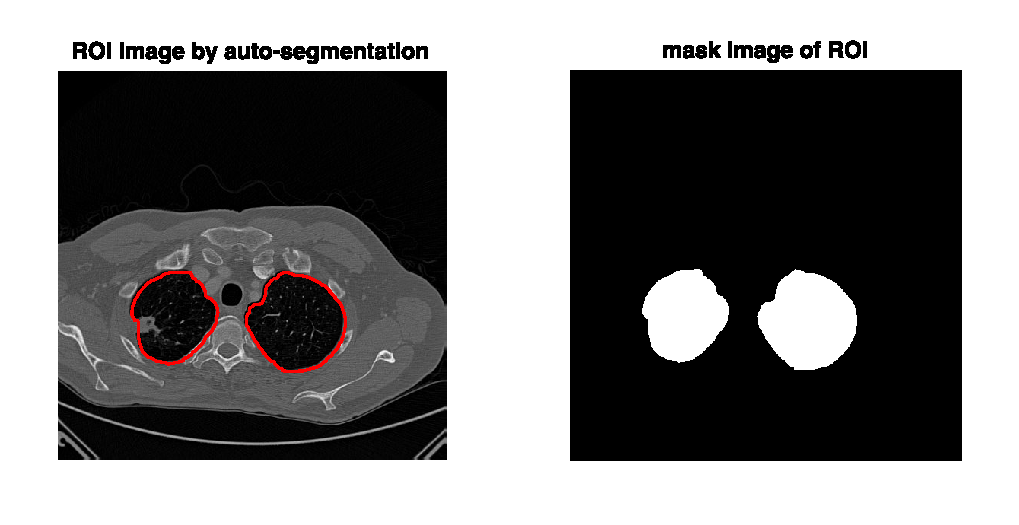
\includegraphics[width=1\linewidth]{ROI}
	\caption{Illustration of ROI in CT image. left: boundary of ROI. right: mask of lung region}
	\label{ROI}
\end{figure}

\section{RESULTS}

\section{FUTURE STEPS}


\addtolength{\textheight}{-12cm}   % This command serves to balance the column lengths
                                  % on the last page of the document manually. It shortens
                                  % the textheight of the last page by a suitable amount.
                                  % This command does not take effect until the next page
                                  % so it should come on the page before the last. Make
                                  % sure that you do not shorten the textheight too much.

%%%%%%%%%%%%%%%%%%%%%%%%%%%%%%%%%%%%%%%%%%%%%%%%%%%%%%%%%%%%%%%%%%%%%%%%%%%%%%%%



%%%%%%%%%%%%%%%%%%%%%%%%%%%%%%%%%%%%%%%%%%%%%%%%%%%%%%%%%%%%%%%%%%%%%%%%%%%%%%%%



%%%%%%%%%%%%%%%%%%%%%%%%%%%%%%%%%%%%%%%%%%%%%%%%%%%%%%%%%%%%%%%%%%%%%%%%%%%%%%%%
\section*{ACKNOWLEDGMENT}



\begin{thebibliography}{99}
 \bibitem{c1} 
%\bibitem{c1} G. O. Young, ?Synthetic structure of industrial plastics (Book style with paper title and editor),? 	in Plastics, 2nd ed. vol. 3, J. Peters, Ed.  New York: McGraw-Hill, 1964, pp. 15?64.
%\bibitem{c2} W.-K. Chen, Linear Networks and Systems (Book style).	Belmont, CA: Wadsworth, 1993, pp. 123?135.
%\bibitem{c3} H. Poor, An Introduction to Signal Detection and Estimation.   New York: Springer-Verlag, 1985, ch. 4.
%\bibitem{c4} B. Smith, ?An approach to graphs of linear forms (Unpublished work style),? unpublished.
%\bibitem{c5} E. H. Miller, ?A note on reflector arrays (Periodical style?Accepted for publication),? IEEE Trans. Antennas Propagat., to be publised.
%\bibitem{c6} J. Wang, ?Fundamentals of erbium-doped fiber amplifiers arrays (Periodical style?Submitted for publication),? IEEE J. Quantum Electron., submitted for publication.
%\bibitem{c7} C. J. Kaufman, Rocky Mountain Research Lab., Boulder, CO, private communication, May 1995.

\end{thebibliography}


\end{document}
